\documentclass[10pt,journal,compsoc]{styles/IEEEtran}
\usepackage{styles/algorithm}
\usepackage[noend]{styles/algorithmic}
\usepackage{graphicx}
\usepackage{color}
\usepackage{listings}
\usepackage{amsmath}
\usepackage[utf8]{inputenc}
\usepackage[T1]{fontenc}
\usepackage[labelformat=empty]{caption}
% *** CITATION PACKAGES ***
\ifCLASSOPTIONcompsoc
  % IEEE Computer Society needs nocompress option
  % requires cite.sty v4.0 or later (November 2003)
  \usepackage[noadjust]{cite}
\else
  % normal IEEE
  \usepackage{cite}
\fi

\title{Tarea 6: M\'etodo de Gradiente Conjugado No Lineal con Half Quadrature Regularization}

\author{Juan Gerardo Fuentes Almeida}

% The paper headers
\markboth{Tarea 6 MÉTODO DE GRADIENTE CONJUGADO}%
{Shell \MakeLowercase{\textit{et al.}}: Bare Advanced Demo of styles/IEEEtran.cls for Journals}

\IEEEtitleabstractindextext{%
\begin{abstract}
En esta pr\'actica se implementa el algoritmo de Gradiente Conjugado No Lineal con Half Quadrature Regularization en el problema de regularizaci\'on de imágenes. Asimismo se hacen comparaciones en tiempo e iteraciones contra diversos m\'etodos de Gradiente Conjugado No Lineal.
\end{abstract}
}

\begin{document}

% make the title area
\maketitle

\IEEEdisplaynontitleabstractindextext

\IEEEpeerreviewmaketitle

\section{Introducci\'on}

\IEEEPARstart{E}l algoritmo de Gradiente Conjugado fue estudiado para minimizar funciones cuadráticas convexas. La version no lineal del método fue adaptado para la minimización de funciones generales convexas y funciones no lineales.\\
 
\section{Teoría}

\subsection{Gradiente Conjugado No Lineal}

\subsubsection{M\'etodo de Fletcher-Reeves (FR)}
El método de Gradiente Conjugado se extiende para funciones no lineales haciendo dos simples cambios al algoritmo Lineal. Primero se reemplaza el calculo del tamaño de paso $\alpha_k$ por una búsqueda en linea que nos permita encontrar un minino de la función no linear $f$ a lo largo de la dirección $p_k$. Segundo, el residuo $r$ es reemplazado por el gradiente de la función no linear $f$\\

\begin{figure}[hbtp]
\centering
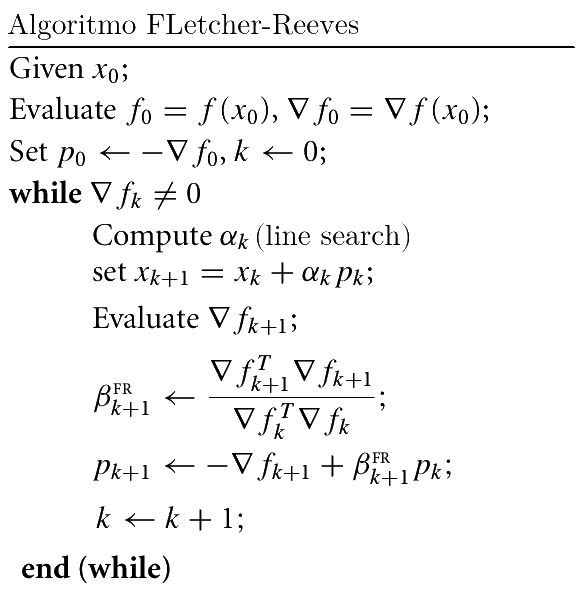
\includegraphics[width=0.35\textwidth]{algoritm.png}
\caption*{}
\end{figure}

Este algoritmo es adecuado para problemas grandes de optimización no lineal porque cada iteración solo requiere la evaluación de la función objetivo y su gradiente. No se requieren operaciones matriciales y se requieren solo una cuantos vectores para almacenamiento. Para asegurar que la dirección $p_k$ sea siempre de descenso hacemos que $\alpha_k$ satisfaga las condiciones fuertes de Wolfe:\\

$\nabla f(x_k+\alpha_k p_k)^Tp_k \geq c_2 \nabla f_k^T p_k$\\

$|\nabla f(x_k+\alpha_k p_k)^Tp_k| \leq c_2| \nabla f_k^T p_k|$\\

donde $0<c_1<c_2<\frac{1}{2}$\\

\subsubsection{M\'etodo de Polak-Ribiere (PR)}

Es una variante importante del método de Fletcher-Reeves, la cual define el parámetro $\beta_k$ como sigue:\\

$\beta_{k+1}^{PR}=\frac{\nabla f_{k+1}^T (\nabla f_{k+1}- \nabla f_{k})}{\nabla f_{k}^T \nabla f_{k}}$\\

Esta $\beta$ es equivalente a la de FR cuando la función es cuadrática y fuertemente convexa, y además la búsqueda en linea es exacta. Sin embargo, en casos generales el comportamiento de ambos algoritmos difiere. Experimentalmente se ha determinado que el algoritmo PR tiende a ser el mas robusto y eficiente.\\

Un hecho acerca del algoritmo PR es que las condiciones fuertes de Wolfe no garantizan que $p_k$ sea siempre una dirección de descenso. Para que esta condición se mantenga se redefine $\beta$ de la siguiente manera:\\

$\beta_{k+1}^{PR+}=max(\beta_{k+1}^{PR},0)$\\

\subsubsection{M\'etodo de Hestenes-Steifel (HS)}

Al igual que el algoritmo de PR, coincide con FR cuando la función es cuadrática y la búsqueda en linea es exacta, se define $\beta$ de la siguiente manera:\\

$\beta_{k+1}^{HS}=\frac{\nabla f_{k+1}^T (\nabla f_{k+1}- \nabla f_{k})}{(\nabla f_{k+1}- \nabla f_{k})^T p_k}$\\

Este algoritmo es similar a PR en términos de convergencia y desempeño.\\

\subsection{Half Quadrature Regularization}

En esta pr\'actica se propone un método de potenciales de regularizaci\'on con preservación de bordes, para lograr esto, implementamos una función potencial a la cual se le agrega un parámetro $k$ de regularizaci\'on de no penalizaci\'on sobre vecinos en los bordes, además del parametro lambda de regularizaci\'on o penalizaci\'on sobre el suavizamiento de vecinos fuera de los bordes:\\

$\rho(U_{r,s})=\omega_s^2 U_{r,s}^2+(1-\omega_s)^2 k$\\

donde $\omega_s$ es la ponderación que se asigna a cada vecino de un pixel, $U_{r,s}=X_r-X_s$ donde $X_r$ representa un pixel de la imagen suavizada y $X_s$ representa un pixel vecino.\\

De esta forma nuestra función objetivo queda definida por el error cuadrático sobre los pixeles de la imagen suavizada con respecto a la imagen observada, m\'as la función potencial sobre los vecinos de cada uno de los pixeles de la imagen:\\

$U(x,y)=\frac{1}{2}\sum\limits_{r \in \Omega}(X_r-Y_r)^2+\frac{\lambda}{2} \sum\limits_{r \in \Omega} \sum\limits_{s \in N_r}\rho(U_{r,s})$\\

\section{Implementaci\'on}

Se implementan versiones de Gradiente Conjugado No Lineal con cada uno de los metodos para el calculo de $\beta$ descritos anteriormente, utilizando Half Quadrature Regularization. Con estas implementaciones se resuelve el problema de suavizamiento o "denoising" mediante la minimización de la función de regularizaci\'on definida por la siguiente expresión:\\

$U(x,y)=\frac{1}{2}\sum\limits_{r \in \Omega}(X_r-Y_r)^2+\frac{\lambda}{2} \sum\limits_{r \in \Omega} \sum\limits_{s \in N_r}\rho(U_{r,s})$\\

donde $N_r$ es la vecindad del pixel $X_r$ de 4 vecinos, $\rho(U_{r,s})$ es la función de regularizaci\'on con $U_{r,s}=X_r-X_s$, $X_r$ es la imagen suavizada, $Y_r$ es la imagen observada con ruido, $r=(i,j)$ son las coordenadas de un pixel, $\Omega$ es el conjunto de pixeles en común a ambas imágenes y $\lambda$ es el parámetro de de regularizaci\'on o penalización.\\

Para maximizar la función definimos la derivada para cierto elemento $r_{ij}$:\\
 
$\frac{\partial}{\partial r_{ij}} U(X,Y)=X_r-Y_r+\lambda \sum\limits_{s \in N_r} \omega_s^2 [X_r-X_s]$

Con la función objetivo definida anteriormente y su vector gradiente, implementamos el algoritmo de Gradiente Conjugado No Lineal, tal como se describe en el pseudoc\'odigo. Para la parte de Half Quadrature Regularization se calcula $\omega_s$ de forma iterativa utilizando Gauss-Seidel, derivando la funci\'on potencial, igualando a cero y obteniendo la siguiente expresi\'on:\\

$\omega_s=\frac{k}{k+U_{r,s}}$\\

Tal como se vio en clase, iniciamos calculando los valores iniciales de la función objetivo y su gradiente, considerando $\omega_s=1$ para todos los vecinos, y una vez obtenida una imagen nueva a partir de la primera, actualizamos los pesos utilizando la formula obtenida anteriormente.\\

\subsection{B\'usqueda en l\'inea}

De acuerdo a las recomendaciones dadas en el libro de referencia, utilizamos las condiciones fuertes de Wolfe para poder garantizar una tamaño de paso que proporcione suficiente descenso. Esta condición se combino con un modelo cuadratico para el calculo de $\alpha_k$.\\

Sin embargo, se tuvieron problemas para lograr implementar un método de búsqueda en linea eficiente a partir de la implementación de la Tarea 2, se observ\'o que en la mayoría de los casos no se obtiene un valor de $\alpha_k$ que cumpla con la condición fuerte de Wolfe. En esos casos, se conserva el valor de $\alpha_k$ que se obtuvo en la iteración anterior.\\


\section{Resultados}

A continuación se muestran las imágenes que se obtuvieron durante la ejecución de la práctica, para diferentes valores de $\lambda$ en una imagen de prueba, utilizando la $\beta$ de Polak-Ribiere:\\

\begin{figure}[H]
	\centering
	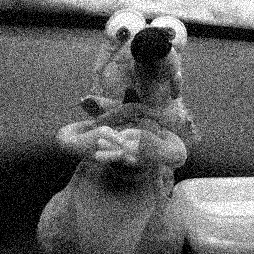
\includegraphics[width=0.15\textwidth]{ardilla.png}
	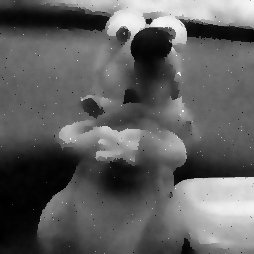
\includegraphics[width=0.15\textwidth]{PR10K400.png}
	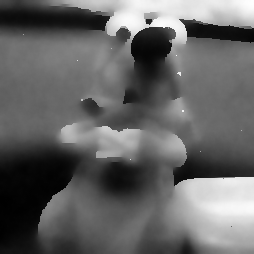
\includegraphics[width=0.15\textwidth]{PR20K400.png}
	
	\caption{Der. a izq.: Imagen observada, $(\lambda,k)=(10,400),(20,400)$}
\end{figure}

\begin{figure}[H]
	\centering
	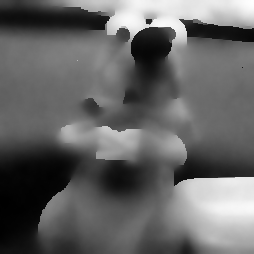
\includegraphics[width=0.15\textwidth]{PR30K400.png}
	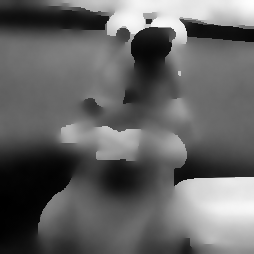
\includegraphics[width=0.15\textwidth]{PR40K400.png}
	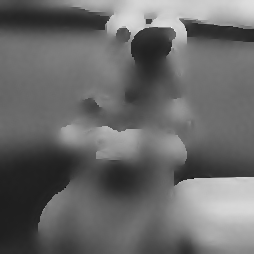
\includegraphics[width=0.15\textwidth]{PR50K400.png}
	
	\caption{Der. a izq.: $(\lambda,k)=(30,400),(40,400),(50,400)$ }
\end{figure}

\begin{figure}[H]
	\centering
	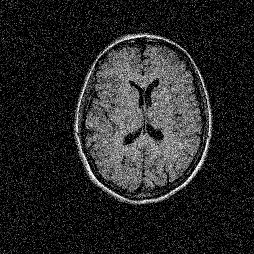
\includegraphics[width=0.15\textwidth]{mri.png}
	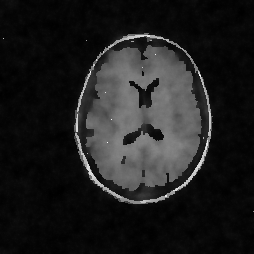
\includegraphics[width=0.15\textwidth]{PR10K4002.png}
	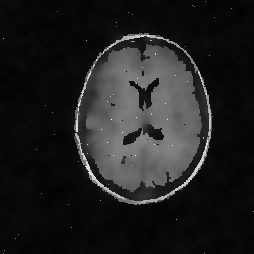
\includegraphics[width=0.15\textwidth]{PR20K4002.png}
	
	\caption{Der. a izq.: Imagen observada, $(\lambda,k)=(10,400),(20,400)$}
\end{figure}

\begin{figure}[H]
	\centering
	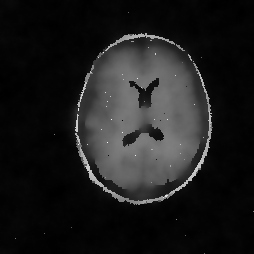
\includegraphics[width=0.15\textwidth]{PR30K4002.png}
	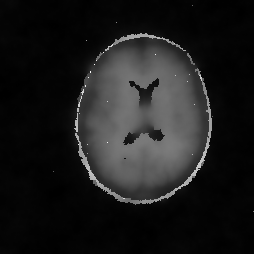
\includegraphics[width=0.15\textwidth]{PR40K4002.png}
	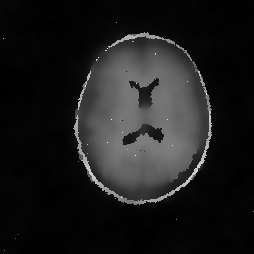
\includegraphics[width=0.15\textwidth]{PR50K4002.png}
	
	\caption{Der. a izq.: $(\lambda,k)=(30,400),(40,400),(50,400)$ }
\end{figure}

El programa implementado en esta práctica recibe el nombre del archivo de la imagen, el parámetro $\lambda$, la constante de regularizaci\'on $k$ y un indicador de la $\beta$ a utilizar (1=Fletcher-Reeves, 2=Polak-Ribiere, 3=Hestenes-Steifel), luego ejecuta los algoritmos de Gradiente Conjugado no Lineal para suavizar la imagen con estos parámetros.\\

Se imprime en pantalla el numero de la iteración, el valor de la función objetivo, los valores de $\alpha$, $\beta$ y el valor de la norma del gradiente para cada iteración. La condición de paro se da a las 500 iteraciones o cuando el valor de la función objetivo varíe en menos de 100 unidades con respecto al valor de la iteración anterior. Se muestra también una tabla donde se comparan cada uno de métodos con relación a su tiempo de ejecución, número de iteraciones y valor de la función objetivo:\\

\begin{figure}[hbtp]
\centering
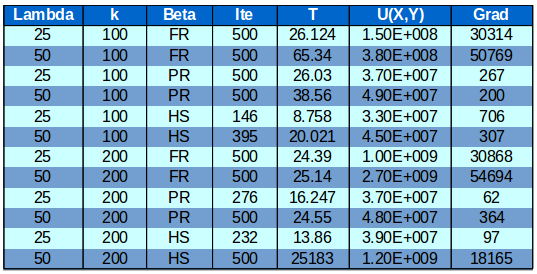
\includegraphics[width=0.5\textwidth]{tabla.png}
\caption{Tabla comparativa entre los algoritmos de Gradiente Conjugado implementados.}
\end{figure}

\section{Conclusiones}

En general se observo durante la pr\'actica que el método de Polak-Ribiere result\'o ser mas eficiente comparado con los demás, lo cual es apoyado por la experimentación mencionada en el libro de referencia, también se observo que resulto complicado obtener un tamaño de paso adecuado para una función no lineal como la que se estuvo tratando. Sorpresivamente se encontró que el método de Fletcher Reeves no result\'o tan bueno como se esperaba, basta con ver la tabla anterior para apreciar que es muy inestable para funciones no lineales y no result\'o ser un minimizador eficiente.\\

\bibliographystyle{plain}
\bibliography{biblio}


\appendix
\section{Implementation details}
El programa est\'a implementado tomando en cuenta todas estandarizaciones indicadas en el curso.

Un \textit{makefile} ha sido generado, el cual soporta los comandos \textit{make}, \textit{run} and \textit{clean}. El programa recibe el nombre del archivo de la imagen, el parámetro $\lambda$, la constante de regularizaci\'on $k$ y un indicador de la $\beta$ a utilizar.

\begin{figure}[hbtp]
\centering
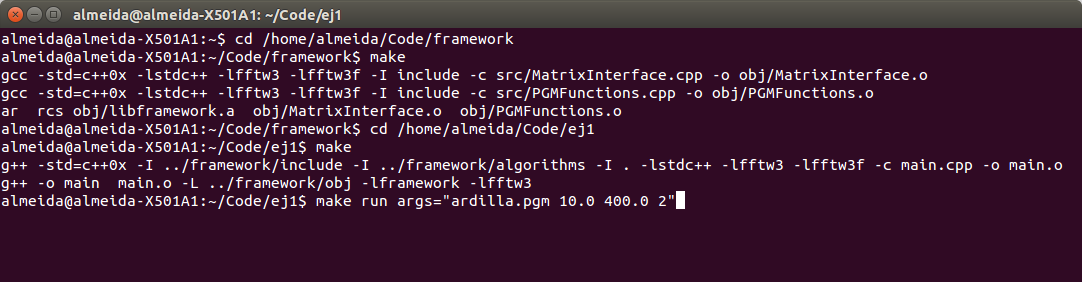
\includegraphics[width=0.5\textwidth]{screen.png}
\caption*{}
\end{figure}

\end{document}


